\documentclass[11pt,class=report,crop=false]{standalone}
\usepackage[screen]{../python}


\begin{document}


%====================================================================
\chapitre{Python : tensorflow avec keras - partie 1}
%====================================================================

\insertvideo{rmxLFqY3--o}{partie 6.1. Utiliser tensorflow}

\insertvideo{hWcYfn4jkO4}{partie 6.2. Tensorflow : exemples à une variable}

\insertvideo{p3smt0Nq-3E}{partie 6.3. Tensorflow : exemples à deux variables}



\objectifs{Le module \Python{} \tensorflow{} est très puissant pour l'apprentissage automatique. Le module \keras{} a été élaboré pour pouvoir utiliser \tensorflow{} plus simplement.
Dans cette partie nous continuons la partie facile : comment utiliser un réseau de neurones déjà paramétré ?}


%%%%%%%%%%%%%%%%%%%%%%%%%%%%%%%%%%%%%%%%%%%%%%%%%%%%%%%%%%%%%%%%%%%%%
\section{Utiliser \tensorflow{} avec \keras}

Le module \keras{} permet de définir facilement des réseaux de neurones en les décrivant couche par couche.
Pour l'instant nous définissons les poids à la main, en attendant de voir plus tard comment les calculer à la machine.
Pour commencer nous allons créer le réseau de neurones correspondant à la figure suivante :

\myfigure{0.9}{
  \tikzinput{fig_pythontf_01}
}


Ceux qui ne veulent pas s'embêter avec les détails techniques peuvent seulement lire la sous-section \ref{ssec:couches} car nous proposerons ensuite un outil simple dans la partie \ref{sec:keras_facile}.


%--------------------------------------------------------------------
\subsection{Module \keras{} de \tensorflow{}}
\label{ssec:keras}

En plus d'importer le module \ci{numpy} (abrégé par \ci{np}), il faut importer le sous-module \ci{keras} du module \ci{tensorflow} et quelques outils spécifiques :

\begin{lstlisting}
from tensorflow import keras
from tensorflow.keras.models import Sequential
from tensorflow.keras.layers import Dense
\end{lstlisting} 


%--------------------------------------------------------------------
\subsection{Couches de neurones}
\label{ssec:couches}

On va définir l'architecture d'un réseau très simple, en le décrivant couche par couche.
\begin{lstlisting}
# Architecture du réseau
modele = Sequential()

# Couches de neurones
modele.add(Dense(2, input_dim=1, activation='relu'))
modele.add(Dense(1, activation='relu'))
\end{lstlisting} 

Explications :
\begin{itemize}
  \item Notre réseau s'appelle \ci{modele}, il est du type \ci{Sequential}, c'est-à-dire qu'il va être décrit par une suite de couches les unes à la suite des autres.\index{tf@\tensorflow/\keras!Sequential@\ci{Sequential}}
  
  \item Chaque couche est ajoutée à la précédente par \ci{modele.add()}.\index{tf@\tensorflow/\keras!add@\ci{add()}}
  L'ordre d'ajout est donc important.
  
  \item Chaque couche est ajoutée par une commande :
  \mycenterline{\ci{modele.add(Dense(nb\_neurones, activation=ma\_fonction))}}
  
  \item Une couche de type \ci{Dense}\index{tf@\tensorflow/\keras!Dense@\ci{Dense()}} signifie que chaque neurone de la nouvelle couche est connecté à toutes les sorties des neurones de la couche précédente.
  
  \myfigure{0.8}{
    \tikzinput{fig_pythontf_02}
  }
 
  
  \item Pour chaque couche, il faut préciser le nombre de neurones qu'elle contient. S'il y a $n$ neurones alors la couche renvoie $n$ valeurs en sortie. On rappelle qu'un neurone renvoie la même valeur de sortie vers tous les neurones de la couche suivante.
  
  \item Pour la première couche, il faut préciser le nombre de valeurs en entrée (par l'option \ci{input_dim = ...}). Dans le code ici, on a une entrée d'une seule variable. Sur la figure ci-dessous un exemple d'une entrée de dimension $3$.

  \myfigure{0.8}{
    \tikzinput{fig_pythontf_03}
  }  

  \item Pour les autres couches, le nombre d'entrées est égal au nombre de sorties de la couche précédente. Il n'est donc pas nécessaire de le préciser.
  
  \item Pour chaque couche, il faut également préciser une fonction d'activation (c'est la même pour tous les neurones de cette couche). Plusieurs fonctions d'activation sont prédéfinies :
  \mycenterline{\ci{'relu'} (ReLU), \quad \ci{'sigmoid'} ($\sigma$), \quad  \ci{'linear'} (identité)}
  Nous verrons plus tard comment définir notre propre fonction d'activation, comme par exemple la fonction marche de Heaviside
  
  \item Notre exemple ne possède qu'une entrée et comme il n'y a qu'un seul neurone sur la dernière couche alors il n'y a qu'une seule valeur en sortie. Ainsi notre réseau va définir une fonction $F : \Rr \to \Rr$, $x \mapsto F(x)$.
  
  \item Mais attention, pour l'instant ce n'est qu'un \emph{modèle} de réseau puisque nous n'avons pas fixé de poids. 

  \myfigure{0.8}{
    \tikzinput{fig_pythontf_04}
  }   

  
  \item Pour vérifier que tout va bien jusque là, on peut exécuter la commande 
  \mycenterline{\ci{modele.summary()}}\index{tf@\tensorflow/\keras!summary@\ci{summary()}}
  qui affiche un résumé des couches et du nombre de poids à définir.
  
\end{itemize}


%--------------------------------------------------------------------
\subsection{Les poids}

Lors de la définition d'un réseau et de la structure de ses couches, des poids aléatoires sont attribués à chaque neurone. 
La démarche habituelle est ensuite d'entraîner le réseau, automatiquement, afin qu'il trouve de \og{}bons\fg{} poids. Pour l'instant, nous continuons de fixer les poids de chaque neurone à la main. 

La commande pour fixer les poids est \ci{set\_weights()}.\index{tf@\tensorflow/\keras!set-weights@\ci{set_weights()}} 

\bigskip

\begin{minipage}{0.55\textwidth}
Voici les poids de la première couche, numérotée $0$ :
\begin{lstlisting}
# Couche 0
coeff = np.array([[1.,-0.5]])
biais = np.array([-1,1])
poids = [coeff,biais]
modele.layers[0].set_weights(poids)
\end{lstlisting}
Définissons les poids de la couche numéro $1$ :
\begin{lstlisting}
# Couche 1
coeff = np.array([[1.0],[1.0]])
biais = np.array([0])
poids = [coeff,biais]
modele.layers[1].set_weights(poids)
\end{lstlisting} 
\end{minipage}
\begin{minipage}{0.40\textwidth}
\myfigure{0.7}{
  \tikzinput{fig_pythontf_01}
}
\end{minipage}


Voici quelques précisions concernant la commande \ci{set\_weights()}. Son utilisation n'est pas très aisée. 
\begin{itemize}
  \item Les poids sont définis pour tous les éléments d'une couche, par une commande \ci{set_weights(poids)}.
  \item Les poids sont donnés sous la forme d'une liste : \ci{poids = [coeff,biais]}.
  \item Les biais sont donnés sous la forme d'un vecteur de biais (un pour chaque neurone).
  \item Les coefficients sont donnés sous la forme d'un tableau à deux dimensions. Il sont définis par entrée. Attention, la structure n'est pas naturelle (nous y reviendrons).
\end{itemize}

Pour vérifier que les poids d'une couche sont corrects, on utilise la commande \ci{get\_weights()}, par exemple pour la première couche :
\mycenterline{\ci{modele.layers[0].get\_weights()}}
\index{tf@\tensorflow/\keras!get-weights@\ci{get_weights()}} 
Cette instruction renvoie les poids sous la forme d'une liste [coefficients,biais] du type :
\mycenterline{\ci{[  [[ 1.  -0.5]],  [-1.  1.]  ]}}

\emph{Astuce !} Cette commande est aussi très pratique avant même de fixer les poids, pour savoir quelle est la forme que doivent prendre les poids afin d'utiliser \ci{set\_weights()}.


%--------------------------------------------------------------------
\subsection{Évaluation}

Comment utiliser le réseau ? C'est très simple avec \ci{predict()}.
\index{tf@\tensorflow/\keras!predict@\ci{predict()}}
 Notre réseau définit une fonction $x \mapsto F(x)$. L'entrée correspond donc à un réel et la sortie également. Voici comment faire :
\begin{lstlisting}
entree = np.array([[3.0]])
sortie = modele.predict(entree)
\end{lstlisting}
Ici \ci{sortie} vaut \ci{[[2.0]]} et donc 
$F(3) = 2$. Ce que l'on peut vérifier à la main en calculant les sorties de chaque neurone.

\myfigure{0.9}{
  \tikzinput{fig_pythontf_05}
}  


%--------------------------------------------------------------------
\subsection{Visualisation}
Afin de tracer le graphe de la fonction $F: \Rr \to \Rr$, on peut calculer d'autres valeurs :

\begin{minipage}{0.64\textwidth}
\begin{lstlisting}
import matplotlib.pyplot as plt
liste_x = np.linspace(-2, 3, num=100)
entree =  np.array([[x] for x in liste_x])

sortie = modele.predict(entree)

liste_y = np.array([y[0] for y in sortie])
plt.plot(liste_x,liste_y)
plt.show()
\end{lstlisting}
\end{minipage}
\begin{minipage}{0.35\textwidth}
\begin{center}
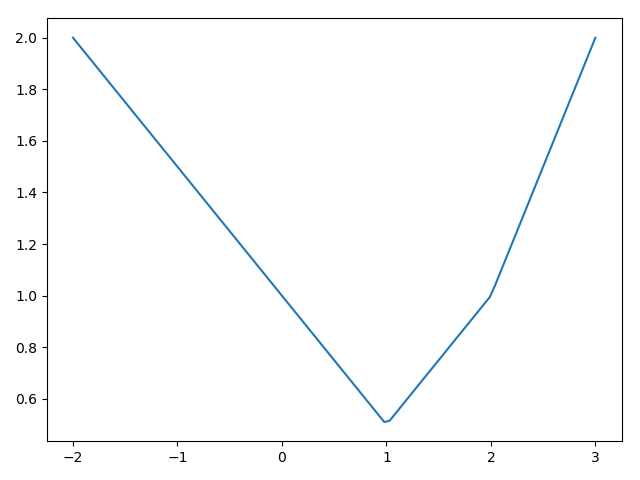
\includegraphics[scale=\myscale,scale=0.4]{figures/pythontf-keras-01}
\end{center}
\end{minipage}

%--------------------------------------------------------------------
\subsection{Autre exemple}

Créons le réseau de neurones ci-dessous :

\myfigure{0.8}{
  \tikzinput{fig_pythontf_06}
} 


\textbf{Couches.}
\begin{lstlisting}
# Architecture du réseau
modele = Sequential()

# Couches de neurones
modele.add(Dense(3, input_dim=2, activation='sigmoid'))
modele.add(Dense(1, activation='sigmoid'))
\end{lstlisting}

La première couche possède $3$ neurones, chacun ayant deux entrées.
La seconde couche n'a qu'un seul neurone (qui a automatiquement $3$ entrées). La fonction d'activation est partout la fonction $\sigma$.

\bigskip
\textbf{Poids.}


\begin{lstlisting}
# Couche 0
coeff = np.array([[1.0,3.0,-5.0],[2.0,-4.0,-6.0]])
biais = np.array([-1.0,0.0,1.0])
poids = [coeff,biais]
modele.layers[0].set_weights(poids)
\end{lstlisting}

Remarquez que les poids ne sont pas définis neurone par neurone, mais par entrée : d'abord les poids de la première entrée pour chaque neurone, puis les poids de la seconde entrée pour chaque neurone, etc.

\begin{lstlisting}
# Couche 1
coeff = np.array([[1.0],[1.0],[1.0]])
biais = np.array([-3.0])
poids = [coeff,biais]
modele.layers[1].set_weights(poids)
\end{lstlisting}

\bigskip
\textbf{Évaluation.}
\begin{lstlisting}
entree = np.array([[7,-5]])
sortie = modele.predict(entree)
\end{lstlisting}

Cette fois l'entrée est du type $(x,y)$ et la sortie correspond à un seul réel $F(x,y)$. Ici $F(7,-5) \simeq 0.123$.

\bigskip
\textbf{Graphique.}
Voici comment tracer le graphe de $F: \Rr^2 \to \Rr$. C'est un peu trop technique, ce n'est pas la peine d'en comprendre les détails.

\begin{minipage}{0.52\textwidth}
\begin{lstlisting}
import matplotlib.pyplot as plt
from mpl_toolkits.mplot3d import Axes3D

VX = np.linspace(-5, 5, 20)
VY = np.linspace(-5, 5, 20)
X,Y = np.meshgrid(VX, VY)
entree = np.c_[X.ravel(), Y.ravel()]

sortie = modele.predict(entree)
Z = sortie.reshape(X.shape)

fig = plt.figure()
ax = plt.axes(projection='3d')
ax.plot_surface(X, Y, Z)
plt.show()
\end{lstlisting}
\end{minipage}
\begin{minipage}{0.47\textwidth}
\begin{center}
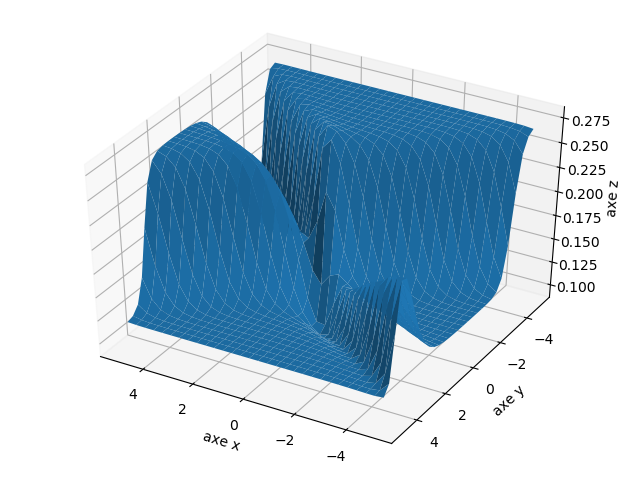
\includegraphics[scale=\myscale,scale=0.5]{figures/pythontf-keras-02a}
\end{center}
\end{minipage}

%%%%%%%%%%%%%%%%%%%%%%%%%%%%%%%%%%%%%%%%%%%%%%%%%%%%%%%%%%%%%%%%%%%%%
\section{Exemples à une variable}
\label{sec:keras_facile}

Comme la philosophie de l'apprentissage automatique n'est pas de définir les poids à la main et que ce cours ne cherche pas à trop entrer dans les détails techniques, nous avons créé spécialement pour vous un autre module : \mycenterline{\ci{keras\_facile}}
afin de définir facilement les poids d'un réseau, d'évaluer des entrées et de tracer le graphe de la fonction associée. Ce module est téléchargeable sur le site du livre avec tous les autres codes sources.

%--------------------------------------------------------------------
\subsection{Exemple simple}

Reprenons l'exemple du réseau de la première partie.

\myfigure{0.8}{
  \tikzinput{fig_pythontf_01}
} 



\begin{lstlisting}
from keras_facile import *

modele = Sequential()
modele.add(Dense(2, input_dim=1, activation='relu'))
modele.add(Dense(1, activation='relu'))

# Poids de la couche 0
# definir_poids(modele,couche,rang,coeff,biais)
definir_poids(modele,0,0,1,-1)  
definir_poids(modele,0,1,-0.5,1)
affiche_poids(modele,0)          # affiche poids de la couche 0

# Poids de la couche 1
definir_poids(modele,1,0,[1,1],0) 
affiche_poids(modele,1) 

# Evaluation
entree = 3
sortie = evaluation(modele,entree)
print('Entrée :',entree,'Sortie :',sortie)

# Affichage graphique
affichage_evaluation_une_var(modele,-2,3)
\end{lstlisting}

C'est tout de même plus simple qu'auparavant !
Bien sûr les résultats sont les mêmes. Ce programme affiche la valeur $F(3) = 2$
et trace directement le graphe de $F$.

\begin{center}
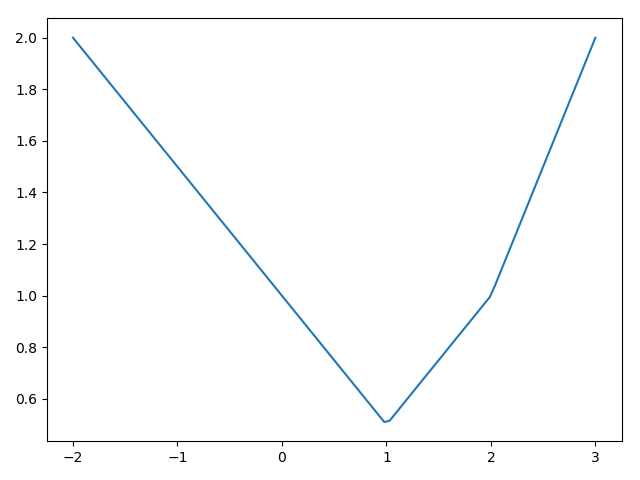
\includegraphics[scale=\myscale,scale=0.4]{figures/pythontf-keras-01}
\end{center}


Le code commence comme précédemment en définissant l'architecture du réseau et les couches.
Ce qui change et qui est plus simple :
\begin{itemize}
  \item La fonction 
  \mycenterline{\ci{definir_poids(modele,couche,rang,coeff,biais)}}
  pour définir les poids d'un neurone à la main. Le neurone est identifié par sa couche, son rang dans cette couche, les coefficients (un nombre \ci{a} ou une liste de nombres \ci{[a1,a2]}, \ci{[a1,a2,a3]}, etc.) et enfin le biais (un nombre).

  \item On vérifie que les poids sont corrects avec \ci{affiche_poids(modele,couche)}.
  On peut aussi fixer tous les poids à zéro avec la fonction \ci{poids_a_zeros(modele,couche)}.

  \item Une fonction d'évaluation 
  \mycenterline{\ci{evaluation(modele,entree)}}
  qui prend en entrées le modèle et un nombre (ou une liste de nombres) et renvoie un nombre.
  C'est une variante simpliste de \ci{modele.predict(entree)}.
  
  \item Une seule commande permet de tracer le graphe !
\end{itemize}

%--------------------------------------------------------------------
\subsection{La fonction marche de Heaviside}

Le module \ci{keras\_facile} définit la fonction marche de Heaviside, que l'on peut ensuite utiliser lors de la déclaration de la couche par l'option :
\mycenterline{\ci{activation = heaviside}}
Attention, il n'y a pas de guillemets autour de \ci{heaviside}.

Voici un réseau d'un seul neurone avec la fonction marche de Heaviside :

\myfigure{1}{
  \tikzinput{fig_pythontf_07}
} 

\begin{lstlisting}
modele = Sequential()
modele.add(Dense(1, input_dim=1, activation=heaviside))
definir_poids(modele,0,0,-0.5,1)
\end{lstlisting}

Voici le graphe de la fonction produite par ce neurone :

\begin{center}
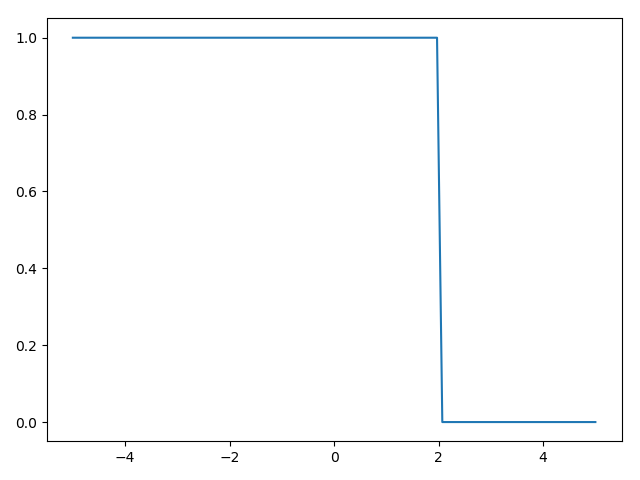
\includegraphics[scale=\myscale,scale=0.4]{figures/pythontf-1var-01}
\end{center}



%--------------------------------------------------------------------
\subsection{Théorème d'approximation universelle}

\index{theoreme@théorème d'approximation universelle}

Enfin, le module \ci{keras\_facile} propose une fonction \ci{calcul_approximation()} qui rend effectif le théorème d'approximation universelle pour les fonctions d'une variable (voir le chapitre \og{}Réseau de  neurones\fg{}).


Prenons l'exemple de la fonction $f : [2,10] \to \Rr$ définie par 
$$f(x) = \cos(2x) + x\sin(3x) + \sqrt{x}$$
que l'on souhaite approcher par un réseau de neurones.


On définit d'abord la fonction $f$, l'intervalle $[a,b]$ et
la précision souhaitée $n$ (l'intervalle $[a,b]$ sera divisé en $n$ sous-intervalles).
Prenons par exemple $a=2$, $b=10$, $n=20$.
\begin{lstlisting}
def f(x):
    return np.cos(2*x) + x*np.sin(3*x) + x**0.5
\end{lstlisting}


Ensuite, on définit un réseau de neurones ayant deux couches, la première avec $2n$ neurones, la seconde avec un seul neurone. Encore une fois, on renvoie au chapitre \og{}Réseau de  neurones\fg{} pour les explications. Ensuite la fonction \ci{calcul_approximation()} calcule les poids qui conviennent pour approcher $f$. 

\begin{lstlisting}
modele = Sequential()

modele.add(Dense(2*n,input_dim=1,activation=heaviside))
modele.add(Dense(1,activation='linear'))

calcul_approximation(modele,f,a,b,n) # calcule et définit les poids
affichage_approximation(modele,f,a,b)
\end{lstlisting}

Une autre fonction trace le graphe de $f$ (en rouge) et la fonction $F$ issue du réseau. Ci-dessous avec $n=5,10,20,50,100$.

\begin{center}
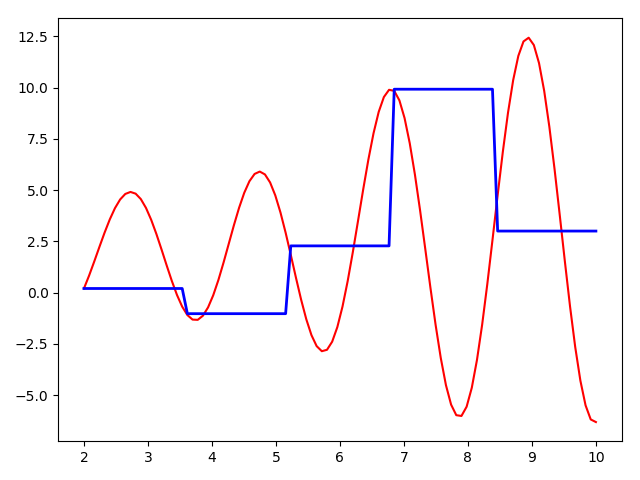
\includegraphics[scale=\myscale,scale=0.45]{figures/pythontf-1var-02a}
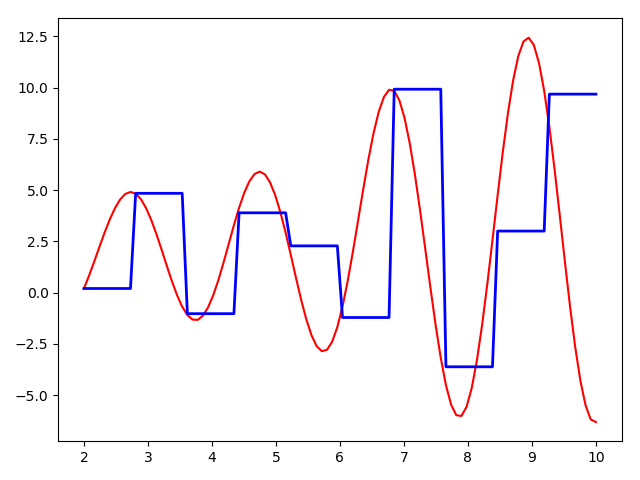
\includegraphics[scale=\myscale,scale=0.45]{figures/pythontf-1var-02b}
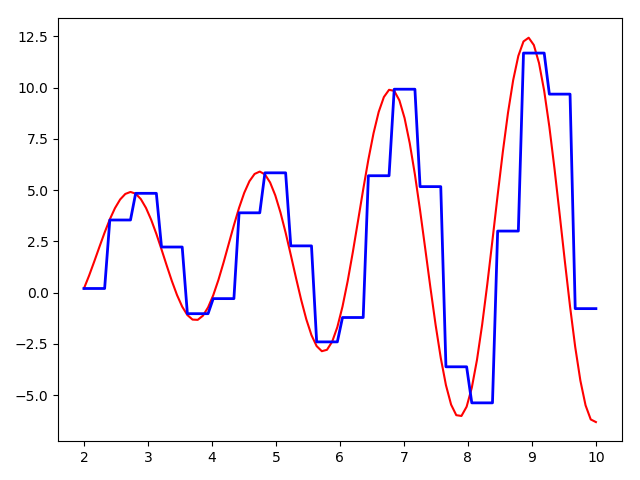
\includegraphics[scale=\myscale,scale=0.3]{figures/pythontf-1var-02c}
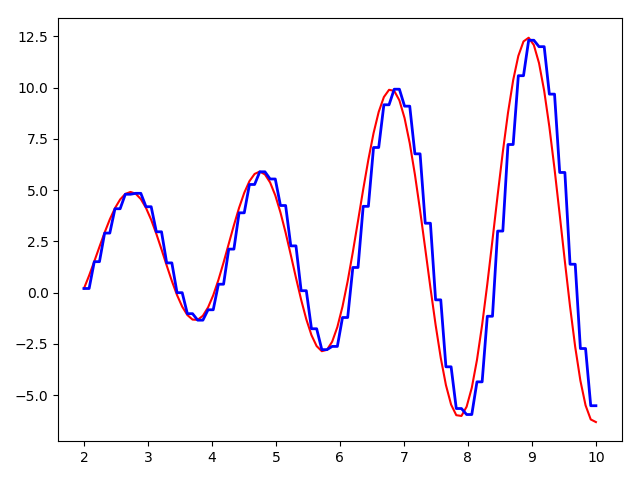
\includegraphics[scale=\myscale,scale=0.3]{figures/pythontf-1var-02d}
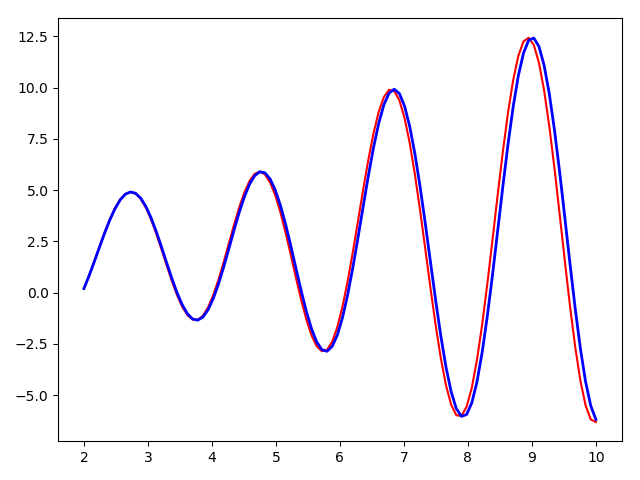
\includegraphics[scale=\myscale,scale=0.3]{figures/pythontf-1var-02e}
\end{center}



%%%%%%%%%%%%%%%%%%%%%%%%%%%%%%%%%%%%%%%%%%%%%%%%%%%%%%%%%%%%%%%%%%%%%
\section{Exemples à deux variables}

%--------------------------------------------------------------------
\subsection{Un exemple avec un seul neurone}


\myfigure{1}{
  \tikzinput{fig_pythontf_08}
} 

Voici la définition de ce neurone :
\begin{lstlisting}
modele = Sequential()
modele.add(Dense(1, input_dim=2, activation='sigmoid'))
definir_poids(modele,0,0,[1,2],-1)
entree = [2.0,1.0]
sortie = evaluation(modele,entree)
\end{lstlisting}
Ici l'entrée est de dimension $2$ du type $(x,y)$. Cela se définit avec \ci{input_dim=2}, il y a donc deux coefficients à définir pour le neurone (ici \ci{[1,2]}) ainsi qu'un biais (ici $-1$).  Enfin, on évalue la fonction $F$ sur un exemple, ici cela donne $F(2,1) \simeq 0.952$.
\begin{lstlisting}
\end{lstlisting}

On termine en affichant le graphe de $F$ dans l'espace et ses lignes de niveau dans le plan, pour $(x,y)$ dans $[-5,5]\times [-5,5]$.
\begin{lstlisting}
affichage_evaluation_deux_var_3d(modele,-5,5,-5,5)
affichage_evaluation_deux_var_2d(modele,-5,5,-5,5)
\end{lstlisting}

\begin{center}
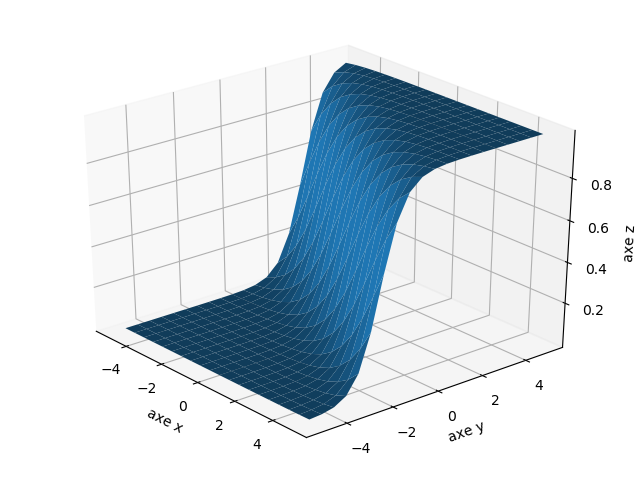
\includegraphics[scale=\myscale,scale=0.5]{figures/pythontf-2var-3d-01}
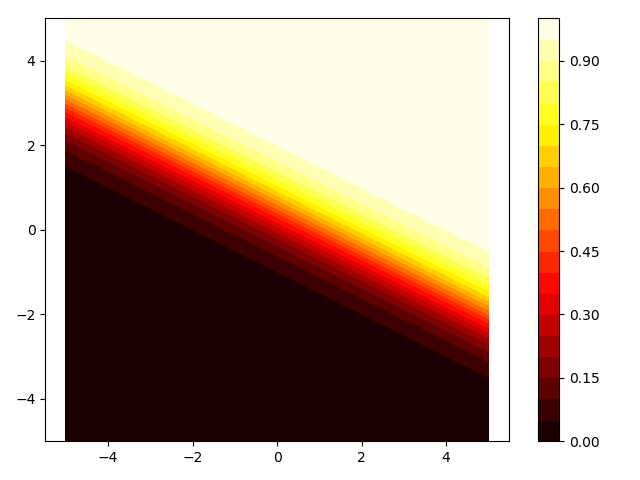
\includegraphics[scale=\myscale,scale=0.4]{figures/pythontf-2var-2d-01}
\end{center}


%--------------------------------------------------------------------
\subsection{Un exemple avec deux couches}

\myfigure{1}{
  \tikzinput{fig_pythontf_09}
} 

\begin{lstlisting}
modele = Sequential()
modele.add(Dense(2, input_dim=2, activation=heaviside))
modele.add(Dense(1, activation=heaviside))
# Couche 0
definir_poids(modele,0,0,[-1,3],0)
definir_poids(modele,0,1,[2,1],0)
# Couche 1
definir_poids(modele,1,0,[1,1],-2) 
\end{lstlisting}

\begin{center}
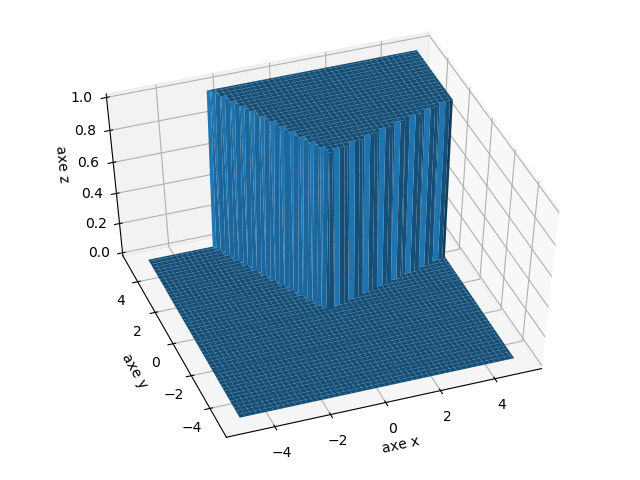
\includegraphics[scale=\myscale,scale=0.5]{figures/pythontf-2var-3d-02}
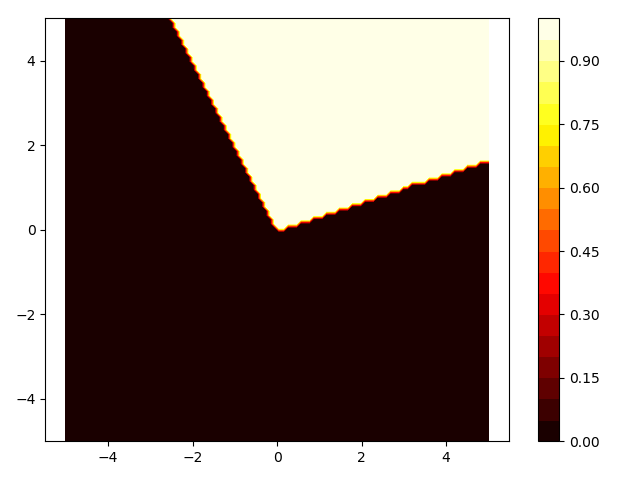
\includegraphics[scale=\myscale,scale=0.4]{figures/pythontf-2var-2d-02}
\end{center}

%%%%%%%%%%%%%%%%%%%%%%%%%%%%%%%%%%%%%%%%%%%%%%%%%%%%%%%%%%%%%%%%%%%%%
\section{Exemples à trois variables}

%--------------------------------------------------------------------
\subsection{Un seul neurone}

\myfigure{1}{
  \tikzinput{fig_pythontf_10}
} 


\begin{lstlisting}
modele = Sequential()
modele.add(Dense(1, input_dim=3, activation='relu'))

definir_poids(modele,0,0,[1,-1,1],-1)
affiche_poids(modele,0)  

entree = [2.0,3.0,4.0]
sortie = evaluation(modele,entree)

affichage_evaluation_trois_var(modele,-5,5,-5,5,-5,5,num=10)
\end{lstlisting}

Ici on obtient $F(2,3,4) = 2$.

L'affichage 3D est plus compliqué à interpréter. Chaque point représente une entrée $(x,y,z)$, la valeur $F(x,y,z)$ est représentée par la couleur du point.
La barre des couleurs donne une idée des valeurs. Ci-dessous les exemples pour $n = 5$ et $n= 10$ sous-intervalles.

\begin{center}
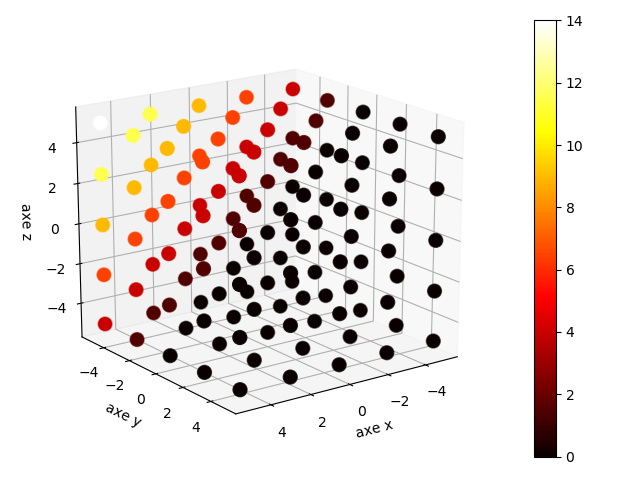
\includegraphics[scale=\myscale,scale=0.5]{figures/pythontf-3var-01a}
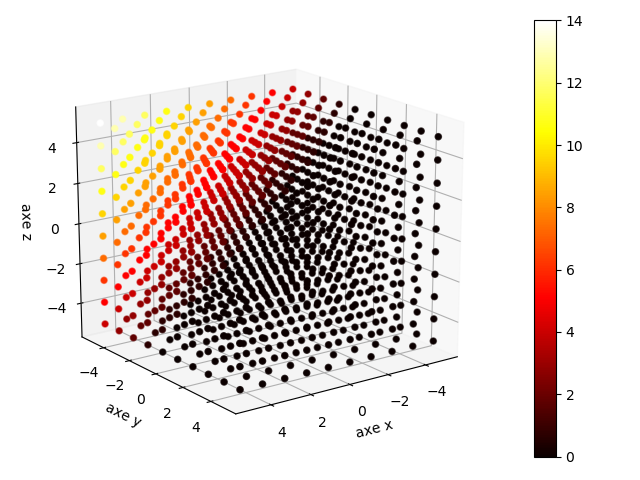
\includegraphics[scale=\myscale,scale=0.5]{figures/pythontf-3var-01b}
% 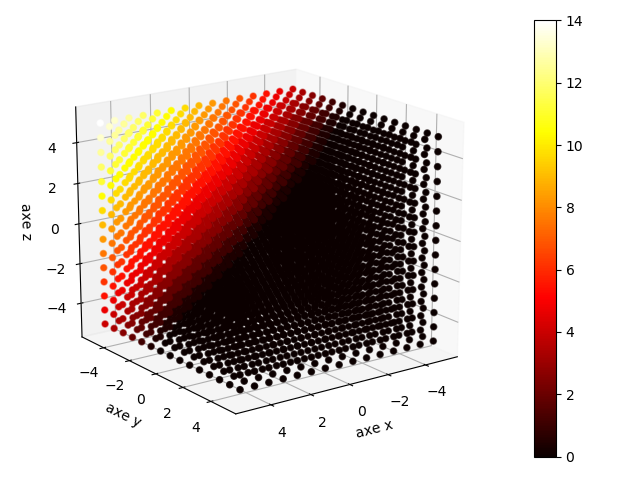
\includegraphics[scale=\myscale,scale=0.5]{figures/pythontf-3var-01c}
\end{center}
%--------------------------------------------------------------------
\subsection{Un réseau pour réaliser un cube}



Voici un réseau plus compliqué et sa représentation graphique (l'absence d'arête signifie un poids nul) :

\myfigure{0.7}{
  \tikzinput{fig_pythontf_11}
} 

La fonction $F(x,y,z)$ prend des valeurs élevées juste autour du point $(0,0,0)$ et des valeurs basses ailleurs (comme une sorte de Soleil positionné en $(0,0,0)$). On note que si on avait choisi la fonction de Heaviside comme fonction d'activation alors la fonction $F$ aurait valu $1$ sur le cube $[-1,1]\times [-1,1]\times[-1,1]$ et $0$ ailleurs. La fonction d'activation $\sigma$ \og{}lisse\fg{} les marches.


\begin{center}
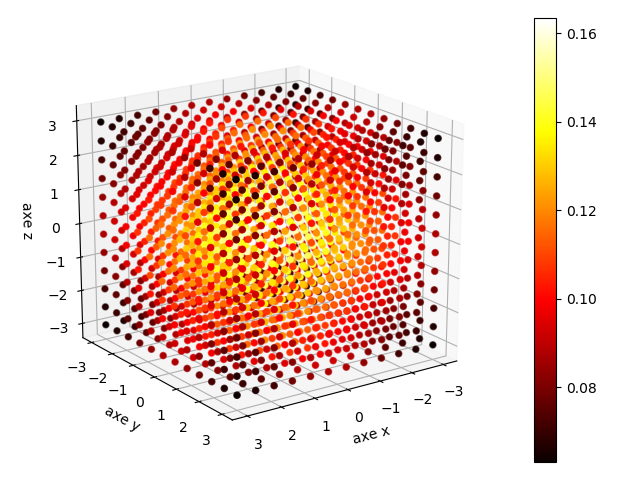
\includegraphics[scale=\myscale,scale=0.7]{figures/pythontf-3var-02}
\end{center}

\end{document}
